\section{迭代三工作项开展流程}
\begin{frame}
    \frametitle{优化SD服务缓存池策略}
    \begin{itemize}
        \item 在之前的单元测试和集成测试工作中,我们小组发现SD绘图的最大开销来源于从硬盘加载用户模型这一过程。因此在迭代三中,我们小组的SD服务维护人员重新设计了模型加载缓存池算法,采用LRU机制,在服务器缓存中维护若干之前用户的模型加载数据结构,并且在缓存池满且缓存未命中时,再从硬盘中将新模型加载到缓存,同时换出LRU队列中最近被加载频度最低的模型数据结构,从而有效提高了对于用户绘图请求的响应速度。在此基础上,我们小组的SD服务维护人员在经过反复的系统测试和实验后,最终将缓存池大小进行了合理设置,从而使得其既能够保证缓存池中的模型可以满足大部分的用户请求场景,同时也不会因为缓存池过大而导致内存占用过高,影响SD服务的运行性能。
    \end{itemize}
\end{frame}

\begin{frame}
    \frametitle{优化SD服务缓存池策略}
    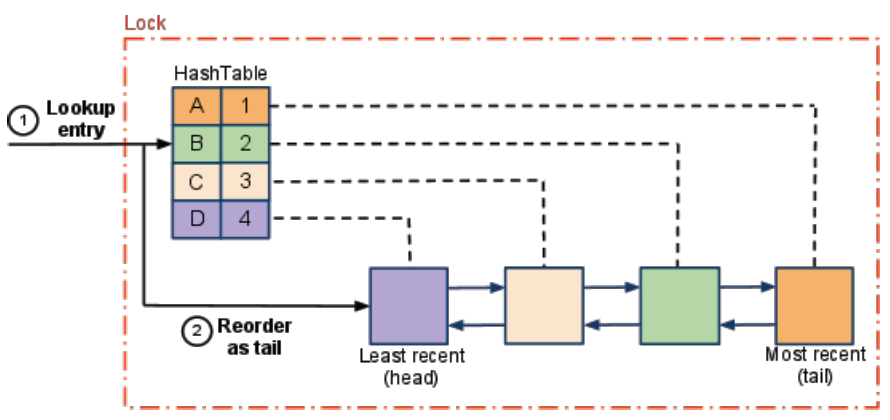
\includegraphics[width=\textwidth]{contents/figure/LRU.png}
\end{frame}